% !TeX root = ../main.tex

\chapter{Fejlesztői dokumentáció}

\section{Követelményelemzés és specifikáció}
A rendszer alapvető célja egy olyan szoftveres megoldás létrehozása, amely képes egy analóg audiojelből zenei metaadatokat és diagnosztikai információkat kinyerni. 

\subsection{Funkcionális követelmények}
\begin{itemize}
    \item \textbf{Valós idejű audio azonosítás:} A rendszernek folyamatosan figyelnie kell a bejövő audio stream-et, és automatikusan detektálnia kell a lejátszás kezdetét. Az észlelés után rögzítenie kell egy rövid audio puffert, és külső audio fingerprinting API-kat kell lekérdeznie a sáv azonosításához.
    \item \textbf{Metaadat-bővítés:} Sikeres audio felismerés után másodlagos adatbázisokat kell lekérdeznie a nagy felbontású albumborítók, a pontos sávhosszúság és a szabványosított albumnév lekéréséhez.
    \item \textbf{Hardverállapot-diagnosztika:} A szoftvernek matematikailag fel kell dolgoznia a hangot a hirtelen felületi pattogások (clicks) detektálására, az alacsony frekvenciás mechanikai motorrezgés (rumble) mérésére, és a magas frekvenciás sziszegő torzítás (sibilance) számszerűsítésére.
    \item \textbf{Hangszedő életciklus kezelés:} Adatbázis fenntartása a felhasználó lemezjátszó tűiről, nyomon követve az aktív hardver kumulatív lejátszási idejét.
    \item \textbf{Digitális hallgatási naplók:} Hitelesítés és automatikus scrobbling külső platformokra (pl. Last.fm).
\end{itemize}

\subsection{Nem-funkcionális követelmények}
\begin{itemize}
    \item \textbf{Teljesítmény és késleltetés:} A háttérben futó audiofeldolgozó szálnak folyamatosan működnie kell anélkül, hogy blokkolná a webszerver műveleteit. 
    \item \textbf{Megbízhatóság és Fallback mechanizmusok:} A hálózati lekérdezéseknek robusztus fallback stratégiákat kell alkalmazniuk. Ha egy elsődleges felismerő motor meghibásodik, a rendszernek meg kell próbálnia a másodlagos források használatát.
    \item \textbf{Adatbázis-konkurencia:} A relációs adatbázisnak támogatnia kell az egyidejű olvasási és írásási műveleteket (Write-Ahead Logging módban).
\end{itemize}

\section{Szoftver architektúra és szerkezet}
A projekt teljes forráskódja nyílt forráskódú, és elérhető a GitHubon: \url{https://github.com/kissdaniel28567/Analog-music-recogniser}. Az alkalmazás egy robusztus kliens-szerver modellt követ. A backend Python nyelven készült, mivel kiterjedt ökoszisztémája (NumPy \cite{numpy}, SciPy \cite{scipy}) ideális a matematikai számításokhoz. A hang rögzítéséhez a \texttt{sounddevice} \cite{sounddevice} könyvtárat alkalmazom. A webszerver réteget a \texttt{Flask} \cite{flask} hajtja meg.
A frontend és a backend közötti állapotmentes kommunikációt a Flask által biztosított RESTful API végpontok valósítják meg. A \ref{tab:api_endpoints}. táblázat foglalja össze az alkalmazás legfontosabb végpontjait és azok funkcióit.

\begin{table}[H]
    \centering
    \renewcommand{\arraystretch}{1.3}
    \begin{tabular}{|c|p{7.5cm}|p{6cm}|}
        \hline
        \textbf{Metódus} & \textbf{Végpont (URL)} & \textbf{Funkció leírása} \\ \hline
        \texttt{POST} & \texttt{/auth/login} & Felhasználó hitelesítése és a munkamenet (session) elindítása. \\ \hline
        \texttt{GET} & \texttt{/api/user/profile} & A hitelesített felhasználó adatainak, hallgatási előzményeinek és regisztrált tűinek lekérése. \\ \hline
        \texttt{POST} & \texttt{/api/user/settings} & Hardveres érzékenységi beállítások (RMS küszöb, pattogás érzékenység) mentése az adatbázisba. \\ \hline
        \texttt{POST} & \texttt{/api/cartridges/\{id\}/update\_limits} & Egy adott hangszedő (tű) várható maximális élettartamának módosítása. \\ \hline
        \texttt{POST} & \texttt{/api/cartridges/\{id\}/reset} & Az aktív hangszedő eddigi kumulatív üzemóráinak nullázása tűcsere esetén. \\ \hline
    \end{tabular}
    \caption{A rendszer alapvető REST API végpontjai és azok funkciói.}
    \label{tab:api_endpoints}
\end{table}


\subsection{Adatbázis Modell}
A perzisztens adattárolást SQLite kezeli SQLAlchemy ORM használatával (lásd \ref{fig:database}. ábra). A \texttt{User} entitás biztosítja az adatok izolációját. A \texttt{Cartridge} tábla követi a tűk üzemóráit, míg a \texttt{TrackHistory} digitális hallgatási naplóként funkcionál. 

\begin{figure}[H]
    \centering
    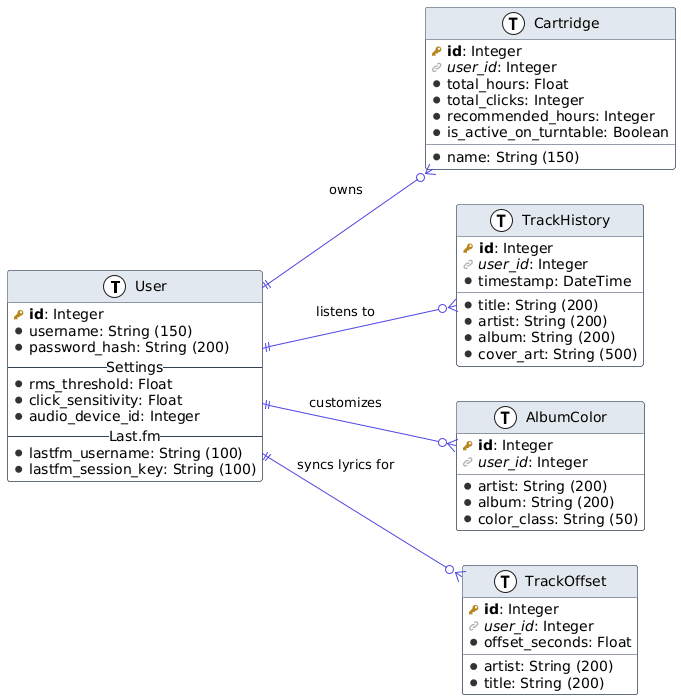
\includegraphics[width=0.85\textwidth]{../Images/database.png}
    \caption{Entity-Relationship Diagram az adatbázis sémájáról.}
    \label{fig:database}
\end{figure}

\subsection{Konkurencia és szálkezelés}
A backend többszálú architektúrát alkalmaz (lásd \ref{fig:sequence}. ábra). Az elsődleges szál folyamatosan olvassa az audio puffert, számítja a diagnosztikát, és megállapítja egy új dal kezdetét. Ekkor elindít egy független másodlagos szálat, amely elvégzi a hálózati kéréseket az audio azonosításhoz, elkerülve az elemzés megfagyását.

\begin{figure}[H]
    \centering
    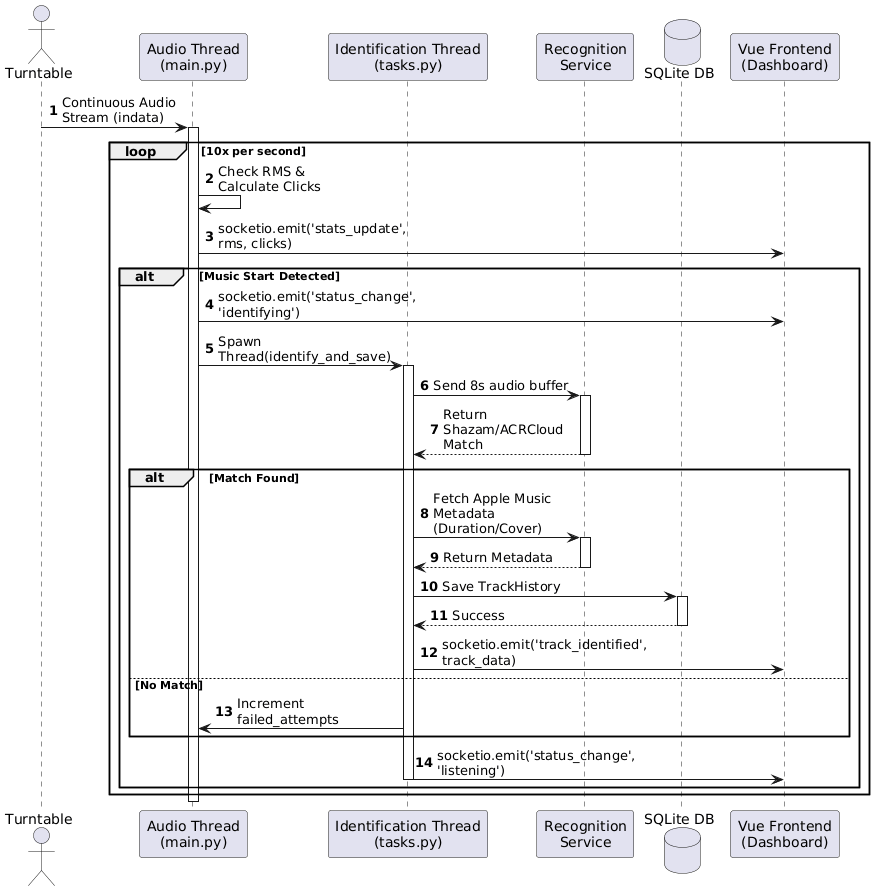
\includegraphics[width=1\textwidth]{../Images/sequence.png}
    \caption{UML Sequence Diagram a többszálú adatfeldolgozásról.}
    \label{fig:sequence}
\end{figure}

\section{Megvalósítási részletek (Backend modulok)}
A rendszer backendje több felelősségi körre van bontva. Az alábbiakban modulonként és metódusonként részletezem a megvalósítást és az alkalmazott matematikai modelleket.

\subsection{Digitális jelfeldolgozás (DSP) -- \texttt{processing.py}}
Ez a modul felelős az analóg audiojel diszkrét matematikai elemzéséért. A \texttt{sounddevice} által rögzített többdimenziós (sztereó) tömböket dolgozza fel másodpercenként többször.

\textbf{1. Effektív hangerőszint (\texttt{calculate\_rms} és \texttt{calculate\_stereo\_rms}):}
A jel energiájának kiszámításához a Root Mean Square (RMS) képletet alkalmazom. A metódus a bejövő lebegőpontos hangminták négyzetes átlagának gyökét veszi:
\begin{equation}
\mathrm{RMS} = \sqrt{\frac{1}{N}\sum_{i=1}^{N} x_i^2}
\end{equation}
Ezt sztereó jelnél a bal és jobb csatornára külön is kiszámítjuk, hogy kivezérlésjelzőt (VU Meter) tudjuk megjeleníteni a kliens oldalon.

\textbf{2. Zeneszám kezdetének detektálása (\texttt{check\_music\_start}):}
Annak megállapítására, hogy a tű a lemezre ért-e, a rendszer figyeli az RMS értéket. Ha ez az érték egy meghatározott küszöb (alapértelmezetten $0.01$) felett marad egy megadott időtartamig (pl. $0.5$ másodperc), a szoftver regisztrálja a lejátszás kezdetét. Ugyanezen elv fordítottjával működik a \texttt{check\_silence\_start} metódus, amely a zeneszámok közötti csendes sávokat ismeri fel.

\textbf{3. Pattogások detektálása (\texttt{detect\_clicks}):}
A bakelitlemezek felületi sérülései hirtelen, magas amplitúdójú tranziensekként (pattanásként) jelentkeznek. A metódus először monósítja a jelet, majd kiszámítja az első deriváltját (két egymást követő minta különbségét), ami felüláteresztő szűrőként funkcionál:
\begin{equation}
d[n] = x[n] - x[n-1]
\end{equation}
Ezután kiszámítom az abszolút deriváltak átlagát ($\mu$) és szórását ($\sigma$). Egy dinamikus küszöbértéket ($T$) állapítok meg, amely egy felhasználó által állítható érzékenységi szorzótól ($k$) függ:
\begin{equation}
T = \mu + k\sigma
\end{equation}
Minden olyan minta, amely meghaladja ezt a küszöböt, statisztikai kiugró értéknek számít, és növeli a pattogásszámlálót.

\textbf{4. Sztereó egyensúly (\texttt{get\_channel\_balance}):}
A lemezjátszó anti-skating beállításának diagnosztikájához a jobb ($R$) és bal ($L$) csatorna RMS értékeiből kiszámítjuk a sztereó egyensúlyt:
\begin{equation}
\text{Balance} = \frac{R - L}{R + L}
\end{equation}
Az eredmény egy $-1$ és $+1$ közötti érték, ahol a $0$ a tökéletes közepet jelenti.

\textbf{5. Mechanikai motorrezgés (\texttt{measure\_rumble}):}
A lemezjátszó motorjának nem kívánt rezgéseit Fast Fourier Transzformációval (FFT) mérjük. A metódus teljes frekvenciatartományba transzformálja a jelet, majd kizárólag a 10 Hz és 50 Hz közötti spektrális energiát összegzi:
\begin{equation}
\text{Rumble} = \sum_{f=10}^{50} |X(f)|
\end{equation}

\textbf{6. Magas frekvenciás torzítás (\texttt{detect\_sibilance}):}
A sibilance (sziszegés) méréséhez a \texttt{SciPy} \texttt{signal.butter} metódusával egy sávszűrőt (Butterworth-sávszűrő \cite{butterworth}) hozunk létre, amely 5 000 Hz és 10 000 Hz között engedi át a jelet. A szűrt jel RMS értékét elosztjuk a teljes jel RMS értékével. Ha ez az arány kirívóan magas, az a tű követési hibájára (tracking distortion) utal.

A fenti algoritmusok stabilitását a fizikai tesztelések során finomhangolt határértékek biztosítják. A \ref{tab:dsp_params}. táblázat foglalja össze az hangelemzés során alkalmazott legfontosabb frekvenciatartományokat és alapértelmezett küszöbértékeket.

\begin{table}[H]
    \centering
    \renewcommand{\arraystretch}{1.3}
    \begin{tabular}{|p{4cm}|p{4.5cm}|p{5.5cm}|}
        \hline
        \textbf{Metrika / Diagnosztika} & \textbf{Frekvenciatartomány} & \textbf{Alapértelmezett küszöbérték / Képlet} \\ \hline
        Zene kezdetének detektálása & Teljes spektrum & $\mathrm{RMS} > 0.01$ (legalább $0.5$ mp hosszan) \\ \hline
        Lejátszás végének (csend) detektálása & Teljes spektrum & $\mathrm{RMS} < 0.01$ (legalább $2.0$ mp hosszan) \\ \hline
        pattogás (Click) detektálás & Magas frekvenciás tranziensek (Derivált jel) & Dinamikus küszöb: $T = \mu + (15 \times \sigma)$ \\ \hline
        Mechanikai rezgés (Rumble) & 10 Hz -- 50 Hz & N/A (A sávhoz tartozó FFT energia összege) \\ \hline
        Sziszegő torzítás (Sibilance) & 5 kHz -- 10 kHz & A szűrt jel RMS aránya a teljes jelhez viszonyítva $> 0.2$ (20\%) \\ \hline
    \end{tabular}
    \caption{A digitális jelfeldolgozás során alkalmazott frekvenciasávok és határértékek.}
    \label{tab:dsp_params}
\end{table}

\pagebreak

\subsection{Zenefelismerés (Recognition) -- \texttt{recognition\_service.py}}
A felismerő modul fejlesztését egy kiterjedt kutatási fázis előzte meg. Három szolgáltatást vizsgáltam: az ACRCloud-ot, az AcoustID-t és a Shazamio-t. Az AcoustID nyílt forráskódú, de a tesztek során kiderült, hogy tiszta audiojelet igényel, így a bakelitre jellemző felületi zajok miatt egyetlen lemezt sem ismert fel. Az ACRCloud pontos volt, de az ingyenes próbaidőszak korlátozásai miatt ipari használatra tervezték.

A végső megoldás a \texttt{Shazamio} \cite{shazamio} könyvtár lett, amely a Shazam aszinkron, visszafejtett (reverse engineered) API-ja. Az \texttt{identify\_audio} metódus aszinkron módon elküld egy 8 másodperces hangmintát a Shazamnak. Ha a Shazam felismeri, visszaadja a szám címét, előadóját és egy Apple Music azonosítót. Ha a Shazam valamilyen oknál fogva hibára fut (fallback), a metódus másodlagos szolgáltatásként az ACRCloud SDK-t használja a felismeréshez.

\subsection{Metaadat-vízesés (Waterfall) -- \texttt{metadata\_service.py}}
A puszta cím és előadó nem elegendő a teljes felhasználói élményhez. Az \texttt{enrich} metódus egy szigorú prioritási sorrendet, úgynevezett vízesés (waterfall) modellt követ a metaadatok beszerzésére.

\begin{enumerate}
    \item \textbf{Apple Music API (\texttt{fetch\_apple}):} Elsődlegesen a Shazam által visszaadott Apple azonosító alapján lekérdezem az iTunes API-t. Ha sikeres, megkapom a pontos sávhosszúságot (milliszekundumban), az album hivatalos nevét és egy nagy felbontású (600x600 px) borítóképet.
    \item \textbf{YouTube Music API (\texttt{fetch\_youtube}):} Ha az Apple Music nem ismeri a dalt, a \texttt{ytmusicapi} segítségével végzek szöveges keresést. Mivel a YouTube alapértelmezetten kis felbontású videó-bélyegképeket ad vissza, az URL manipulálásával (\texttt{w120-h120} cseréje \texttt{w1000-h1000}-re) kényszerítem ki a jó minőségű képet.
    \item \textbf{MusicBrainz Fallback (\texttt{fetch\_musicbrainz\_cover}):} Ha a YouTube Music sem ad megfelelő borítót, harmadik lépcsőként a CoverArtArchive REST API-ját hívom meg az előadó és az album neve alapján.
\end{enumerate}

\begin{figure}[H]
    \centering
    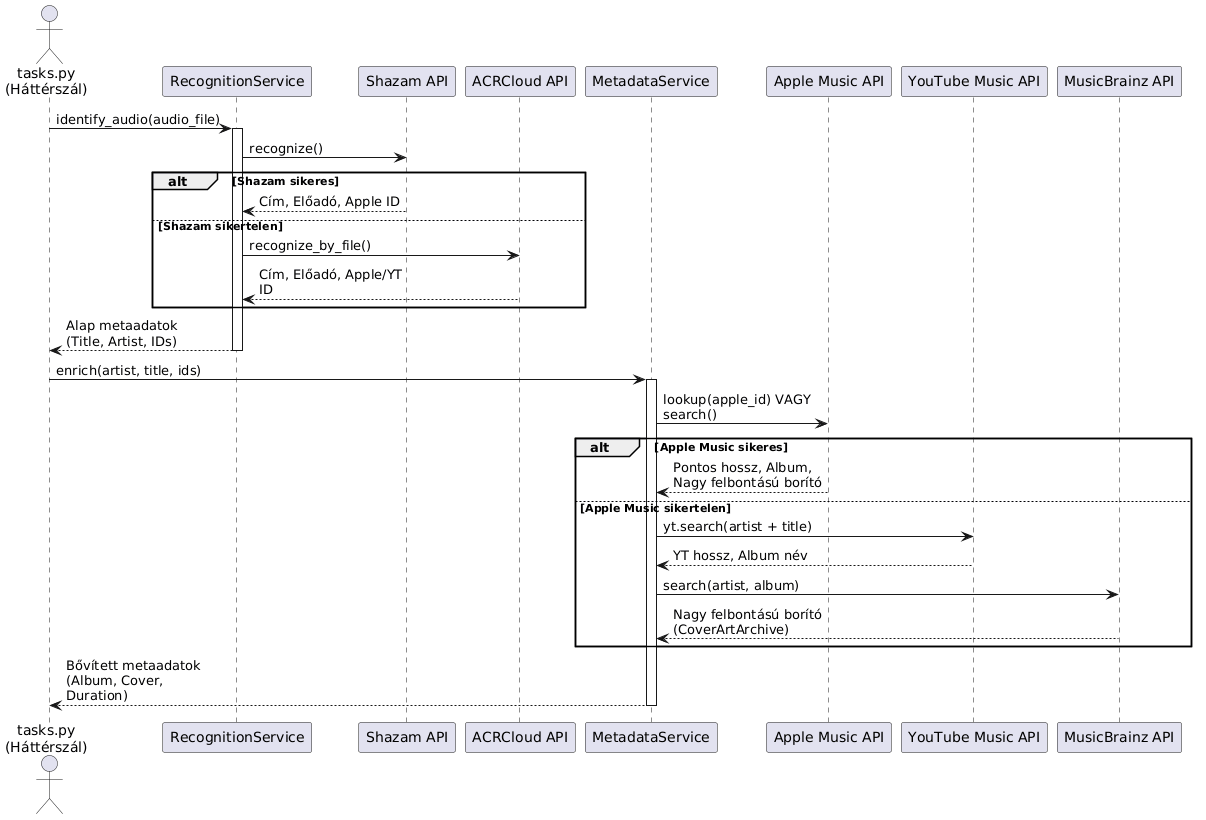
\includegraphics[width=0.85\textwidth]{../Images/fallback_diagram.png}
    \caption{A Fallback és Metaadat-vízesés folyamata (UML Sequence Diagram).}
    \label{fig:fallback}
\end{figure}

\subsection{Háttérfolyamatok és Szálkezelés -- \texttt{tasks.py}}
A valós idejű működés magját az \texttt{audio\_processing\_thread} háttérszál adja. Ez a szál egy végtelen ciklusban, 4096 mintás blokkokban (chunk) olvassa a hangkártya bemenetét. Minden blokkon lefuttatja a korábban említett DSP metódusokat (RMS, click, rumble, sibilance). 

Az I/O műveletek optimalizálása érdekében a szál egy \texttt{buffer\_seconds} memóriaváltozóban halmozza fel a lejátszott időt, és csak 10 másodpercenként írja az adatbázisba (\texttt{Cartridge} kopás mentése). Minden iteráció végén a szál a \texttt{SocketIO} csatornán keresztül egy \texttt{stats\_update} eseményben közvetíti az élő adatokat a kliensnek.

Amikor a DSP modul megállapítja egy új dal kezdetét, a rendszer elindítja az \texttt{identify\_and\_save} metódust egy külön szálon. Ez:
\begin{enumerate}
    \item Rögzít 8 másodpercnyi hangot (\texttt{AudioCapture}).
    \item Meghívja a \texttt{RecognitionService}-t.
    \item Meghívja a \texttt{MetadataService}-t.
    \item Hálózati lekérdezést indít a \texttt{lrclib.net} API felé, hogy letöltse az időbélyeggel ellátott dalszöveget.
    \item Elmenti a sikeres találatot a \texttt{TrackHistory} adatbázis táblába.
\end{enumerate}
Végül, a lejátszás során egy figyelő logika vizsgálja, hogy a sáv eltelt ideje elérte-e az 50\%-ot (vagy a 4 percet). Ha igen, a \texttt{scrobble\_track\_async} háttérfolyamat aszinkron módon regisztrálja a lejátszást a felhasználó Last.fm fiókjában.

\section{Tesztelés és Értékelés}

\subsection{Automatizált Egységtesztelés (Unit Testing)}
A rendszer stabilitásának és hosszú távú karbantarthatóságának biztosítása érdekében a Python beépített \texttt{unittest} keretrendszerével átfogó automatizált egységteszteket (Unit Tests) írtam. Mivel az alkalmazás fizikai hardverekkel (lemezjátszó, hangkártya) és külső webes API-kkal is kommunikál, a tesztelés során kiemelt feladat volt ezeknek a külső függőségeknek a szimulálása (Mocking) és izolálása. A tesztek logikailag három fő kategóriába sorolhatók:

\textbf{1. Adatbázis és API végpontok tesztelése (\texttt{test\_api.py}):}
A REST API és az adatbázis-modellek teszteléséhez a Flask keretrendszer teszt-kliensét (\texttt{test\_client}) használtuk. Annak érdekében, hogy a tesztek futtatása ne tegye tönkre a valós, éles adatbázisban tárolt felhasználói adatokat, a tesztkörnyezet egy memóriában futó SQLite adatbázist (\texttt{sqlite:///:memory:}) inicializál. Ez a memóriabázis a tesztek lefutása után azonnal megsemmisül.
A tesztek során szimuláltam a kliens bejelentkezését (\texttt{POST /auth/login}), ellenőriztem a jogosultságkezelést (nem hitelesített kérések elutasítása 401-es hibakóddal), valamint teszteltem a hardveres beállítások és a hangszedő limitjeinek sikeres módosítását.

\textbf{2. Digitális Jelfeldolgozás szimulálása (\texttt{test\_audio\_dsp.py}):}
A DSP algoritmusok pontosságának igazolásához nem volt szükség valós fizikai hanglemezek lejátszására a tesztkörnyezetben. Ehelyett a \texttt{NumPy} könyvtár segítségével szintetikus (mesterségesen generált) matematikai tömböket hoztam létre, amelyek egy tökéletes hangkártya kimenetét imitálják:
\begin{itemize}
    \item \textbf{Csend és Konstans jelek:} Egy teljesen nullákkal feltöltött tömbbel (\texttt{np.zeros}) igazoltam, hogy a rendszer pontosan 0.0 RMS értéket ad vissza, egy fix értékekkel feltöltött tömbbel pedig a matematikai átlagolás helyességét ellenőriztem.
    \item \textbf{pattogás (Click) szimuláció:} Egy csendes tömb közepébe egyetlen masszív értéket (tüskét) injektáltam (\texttt{audio\_chunk[2000] =[1.0, 1.0]}). Az algoritmus sikeresen megtalálta a statisztikai kiugrást.
    \item \textbf{Frekvencia-generálás (Rumble és Sibilance):} A frekvenciaszűrők teszteléséhez szinuszgörbéket generáltam a matematikai képlet ($ \sin(2 \pi \cdot f \cdot t) $, ahol $f, t \in \mathbb{R}$) alapján. Egy tiszta 30 Hz-es szinuszhullámot generálva a \texttt{measure\_rumble} metódus vártan magas motorrezgés-értéket mutatott, míg egy 8000 Hz-es (8 kHz) szinuszhullám sikeresen triggerelte a \texttt{detect\_sibilance} (sziszegés) mérőeszközt, igazolva a Butterworth-sávszűrő hibátlan működését.
\end{itemize}

\textbf{3. Külső szolgáltatások izolálása Mocking-gal (\texttt{test\_services.py}):}
A harmadik féltől származó API-kat (Apple Music, YouTube Music, Last.fm) hívó szolgáltatások tesztelése speciális kihívást jelentett. Nem engedhető meg, hogy a tesztek futtatása valós hálózati forgalmat generáljon (ami terhelné az API-kat, vagy internet hiányában a tesztek elbukását okozná). Ezt a problémát a Python \texttt{unittest.mock.patch} dekorátorával oldottam meg.

A szimuláció (Mocking) során a kód elhiteti a szolgáltatással, hogy a hálózati kérés lefutott. Amikor például a rendszer meghívja az \texttt{urllib.request.urlopen} metódust, a @patch megállítja a kérést, és egy előre megírt, mesterséges (fake) JSON választ ad vissza (lásd \ref{fig:mocking}. ábra). Ezzel a módszerrel sikeresen leteszteltem:
\begin{itemize}
    \item A \textbf{Waterfall (Vízesés) metaadat-logikát}, megfigyelve, hogy az algoritmus valóban továbblép-e a YouTube keresésre, ha az Apple Music szimulált válasza üres.
    \item A dalszövegek (LRC) reguláris kifejezésekkel (Regex) történő időbélyeg-feldolgozását (\texttt{\lbrack MM:SS.xx\rbrack}).
    \item A Last.fm scrobbling folyamatot, ahol a hálózati réteget teljes egészében szimulált \texttt{MagicMock} objektumokkal helyettesítettem, vizsgálva, hogy a belső logika az API szervereinek elérhetetlensége esetén is biztonságosan, összeomlás nélkül lefut.
\end{itemize}

\begin{figure}[H]
    \centering
    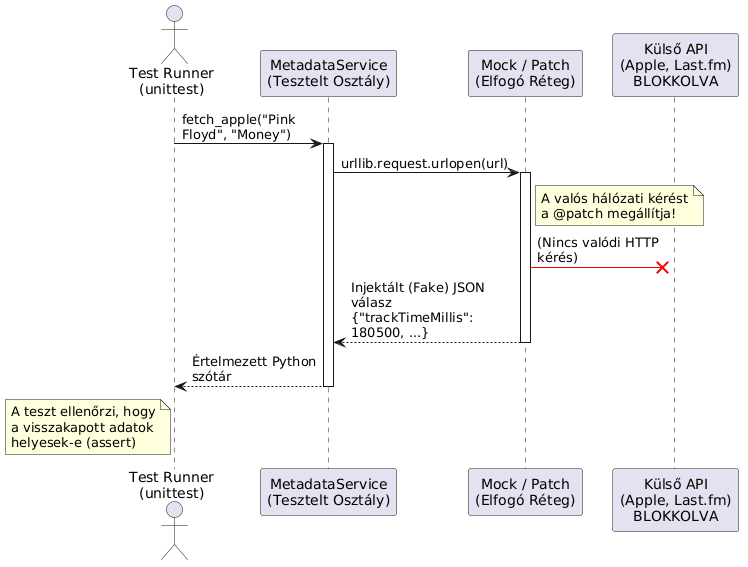
\includegraphics[width=0.85\textwidth]{../Images/mock_diagram.png}
    \caption{UML Sequence Diagram a külső API-k @patch alapú szimulálásáról (Mocking).}
    \label{fig:mocking}
\end{figure}

Az automatizált egységtesztek által lefedett üzleti logikát és elvárt viselkedéseket a \ref{tab:test_user_stories}. táblázat foglalja össze felhasználói történetek (User Stories) formájában.

\renewcommand{\arraystretch}{1.3}
\footnotesize

\begin{longtable}{|p{3.2cm}|p{3.6cm}|p{3.2cm}|p{4cm}|}
    \caption{Az automatizált egységtesztek (Unit Tests) által lefedett folyamatok Given-When-Then formátumban.}
    \label{tab:test_user_stories} \\
    \hline
    \textbf{Teszteset / Modul} & \textbf{Feltétel (Given)} & \textbf{Esemény (When)} & \textbf{Várt Eredmény (Then)} \\ \hline
    \endfirsthead

    \multicolumn{4}{c}{{\tablename\ \thetable{} -- folytatás az előző oldalról}} \\
    \hline
    \textbf{Teszteset / Modul} & \textbf{Feltétel (Given)} & \textbf{Esemény (When)} & \textbf{Várt Eredmény (Then)} \\ \hline
    \endhead

    \hline
    \multicolumn{4}{|r|}{\textit{Folytatás a következő oldalon...}} \\ \hline

    \hline
    \endlastfoot

    \multicolumn{4}{|c|}{\textbf{REST API és Adatbázis Modellek (\texttt{test\_api.py})}} \\ \hline
    \texttt{login\_success} \newline \texttt{login\_failure} & Érvényes vagy érvénytelen hitelesítő adatok. & A kliens bejelentkezési (\texttt{POST}) kérést küld a végpontra. & \texttt{200 OK} és User ID visszatérés / \texttt{401 Unauthorized} hiba. \\ \hline
    \texttt{get\_profile\_...} & Hitelesített vagy munkamenet nélküli állapot. & A kliens lekéri a profiladatokat (\texttt{GET}). & Hiánytalan JSON profil struktúra visszaadása / \texttt{401}-es megtagadás. \\ \hline
    \texttt{update\_settings} & Hitelesített munkamenet és új hardveres szenzoradatok. & A hardver beállítások mentése (\texttt{POST}) megtörténik. & Az RMS és érzékenységi értékek sikeresen frissülnek az adatbázisban. \\ \hline
    \texttt{cartridge\_...} & Hitelesített kliens, érvényes aktív hangszedő. & Limit módosítási vagy óra nullázási (Reset) kérés érkezik. & A hangszedő limitje frissül, az üzemóra pedig pontosan \texttt{0.0}-ra áll át. \\ \hline

    \multicolumn{4}{|c|}{\textbf{Digitális Jelfeldolgozás (\texttt{test\_audio\_dsp.py})}} \\ \hline
    \texttt{rms\_perfect\_silence} \newline \texttt{rms\_constant\_signal} & Tökéletes csend (nullákból álló tömb) vagy konstans jelszint. & Az RMS algoritmus kiszámítja az effektív hangerőt. & Csend esetén pontosan \texttt{0.0} / Konstans esetén az elvárt állandó érték. \\ \hline
    \texttt{click\_detection...} & Csendes szintetikus hangminta egyetlen masszív tüskével. & Felületi pattogás (Click) detektálás futtatása. & A statisztikai algoritmus megtalálja a kiugrást (clicks $>0$). \\ \hline
    \texttt{stereo\_rms...} \newline \texttt{channel\_balance...} & Féloldalas (csak egyik csatornán aktív) vagy középre zárt hang. & Sztereó szétválasztás és egyensúly (balance) számítás. & Csatornánkénti helyes RMS érték, negatív vagy pontosan \texttt{0.0} egyensúly. \\ \hline
    \texttt{measure\_rumble...} & Injektált tiszta 30 Hz-es alacsony frekvenciás szinuszhullám. & Motorrezgés (Rumble) mérése az FFT spektrumon. & Válaszként nagyon magas (>1000) rezgésenergia érték. \\ \hline
    \texttt{detect\_sibilance...} & Injektált tiszta 8 kHz-es magas frekvenciás szinuszhullám. & Sziszegés (Sibilance) mérése sávszűrőn keresztül. & Magas ($\sim 1.0$) torzítási arány, a szűrő sikeresen átengedi a jelet. \\ \hline

    \multicolumn{4}{|c|}{\textbf{Külső API-k és Fallback Logika (\texttt{test\_services.py})}} \\ \hline
    \texttt{enrich\_waterfall...} & Az Apple Music API ad találatot, vagy egyáltalán nem ad találatot. & Metaadat dúsítás (Enrich Waterfall) indítása. & Apple találat esetén azonnali visszatérés / Nincs találat esetén fallback a YouTube felé. \\ \hline
    \texttt{youtube\_duration...} & \texttt{"MM:SS"} / \texttt{"HH:MM:SS"} formátum vagy feldolgozhatatlan string. & YouTube formátumú időtartam konvertálása másodpercre. & Helyes számított másodperc érték / Szemét adatnál 210 mp biztonsági fallback. \\ \hline
    \texttt{lrc\_regex...} & Szinkronizált, normál szöveges, vagy üres sorokat tartalmazó LRC. & Dalszöveg időbélyeg (Regex) feldolgozása. & Helyes lebegőpontos mp / Nincs szinkron esetén \texttt{-1} mp / Üres sor átugrása. \\ \hline
    \texttt{fetch\_apple\_...} & Szimulált JSON válasz / Üres találat / Hálózati hiba API leálláskor. & Apple Music metódus \texttt{@patch} hívása (Mocking). & Pontos album, borító kinyerése / Hiba esetén biztonságos \texttt{None} visszatérés. \\ \hline
    \texttt{fetch\_youtube\_...} & Szimulált YT Music JSON válasz valid adatokkal. & YouTube keresési metódus hívása. & Kép URL manipulálása (w1000-h1000) és nagy felbontású borító kinyerése. \\ \hline
    \texttt{lastfm\_scrobble...} \newline \texttt{lastfm\_session...} & Érvényes Last.fm token / Hálózati szakadás / Érvényes Session Key. & Session kulcs csere és Scrobble hívás indítása. & Sikeres Session Key kinyerés / Scrobble futtatása / API hiba csendes elkapása. \\ \hline

\end{longtable}

\subsection{Frontend renderelés, Vizuális Megjelenítés és Témázás}
A felhasználói felület (UI) megjelenítése a letisztult elrendezés mellett a személyre szabhatóságra fókuszál. Az egyedi stíluslapok (\texttt{themes.css}, \texttt{dashboard.css}) segítségével a rendszer vizuálisan is alkalmazkodik a felhasználó preferenciáihoz.

\textbf{Dinamikus Témaváltás (Modern vs. Retro):}
Az alkalmazás megjelenését a gyökér (\texttt{:root}) elemen definiált CSS változók vezérlik, amelyeket a HTML DOM-on (Document Object Model) lévő \texttt{data-theme} és \texttt{data-style} attribútumok manipulálnak. 
\begin{itemize}
    \item A \textbf{Modern} stílus (\texttt{data-style="modern"}) lekerekített sarkokat (\texttt{--modern-radius}), finom árnyékokat és lágy átmeneteket használ a kivezérlésjelzőknél (függőleges LED sávok).
    \item A \textbf{Retro} stílus (\texttt{data-style="retro"}) ezzel szemben a klasszikus Windows 95/98 esztétikát idézi: éles sarkok (\texttt{0px} border-radius), \texttt{inset/outset} dobozárnyékok (bevel effect), klasszikus analóg mutatós VU méterek, és monospace (Courier New) tipográfia.
\end{itemize}

\textbf{A Bakelitlemez Renderelése és Animációja:}
A forgó lemez vizuális illúzióját tiszta CSS megoldások adják, elkerülve a memóriaintenzív 3D renderelést.
\begin{itemize}
    \item \textbf{Textúrák és Színek:} A lemez alapját több, mint 30 választható CSS osztály adja. Választhatunk egyszerű és összetett színek közül. Az összetettebb, több színű lemezek matematikai színátmenetekkel készülnek, például a \textit{Rasta Split} lemez egy \texttt{conic-gradient(\#e20613 0 120deg, \#f9e514 120deg 240deg...)} kód segítségével osztja a kört három egyenlő cikkelyre. Más komplex mintákat (pl. \textit{Galaxy Splash}) nagy felbontású ismétlődő háttérképek (\texttt{background: url(...)}) adnak.
    \item \textbf{A Barázdák illúziója:} A hanglemez textúrájára egy \texttt{::after} pszeudo-elem borul, amely egy \texttt{repeating-radial-gradient} segítségével koncentrikus, finoman átlátszó köröket rajzol, tökéletesen imitálva a fizikai barázdákat. Mivel ezen az elemen \texttt{pointer-events: none} van, a felhasználó gond nélkül tud kattintani a lemezre.
    \item \textbf{Forgás (Rotation):} Amikor az audio elemző zenét detektál, a Vue keretrendszer dinamikusan rárakja a DOM elemre a \texttt{spinning} osztályt. Ez egy végtelenített CSS \texttt{@keyframes spin} animációt indít el, amely 4 másodperc alatt forgatja körbe (\texttt{transform: rotate(360deg)}) a lemezt.
\end{itemize}

\subsection{Kliens-oldali Logika és Állapotkezelés (useDashboard.js)}
A Főképernyő (Dashboard) mögötti reaktív logikát a Vue 3 Composition API-ra épülő \texttt{useDashboard} és \texttt{useVinylInteractions} modulok kezelik. A legfontosabb folyamatok és metódusok a következők:

\textbf{1. Socket.IO kommunikáció és adatszinkronizáció:}
\begin{itemize}
    \item \texttt{onMounted}: A komponens betöltésekor inicializálja a WebSocket kapcsolatot a backend-del. Három fő eseményre (event) iratkozik fel: \texttt{stats\_update}, \texttt{status\_change}, és \texttt{track\_identified}.
    \item \texttt{stats\_update} figyelő: Másodpercenként többször lefut. Frissíti a Vue reaktív (\texttt{ref}) változóit: az RMS értékeket (L/R kivezérlés), a lejátszási időt (\texttt{trackTime}), a mechanikai zajokat (\texttt{currentRumble}, \texttt{currentSibilance}), és betölti az aktuális pattogásokat a \texttt{clickHistory} tömbbe az idővonal megrajzolásához.
    \item \texttt{status\_change} figyelő: Kezeli a felület ``Keresés folyamatban'' (Identifying...) állapotát, blokkolva a felhasználói interakciókat a keresés alatt.
    \item \texttt{track\_identified} figyelő: Sikeres találat esetén betölti a borítóképet, és azonnal meghívja a dalszöveg-feldolgozó rutint, majd a képernyőt a megfelelő sorhoz görgeti.
    \item \texttt{onUnmounted}: Biztonságosan lezárja a socket kapcsolatot (\texttt{socket.disconnect()}), amikor a felhasználó elhagyja az oldalt, megelőzve a memóriaszivárgást.
\end{itemize}

\textbf{2. Dalszöveg (Lyrics) feldolgozása és szinkronizációja:}
\begin{itemize}
    \item \texttt{parseLRC}: Reguláris kifejezések (Regex: \texttt{\textbackslash[\textbackslash d\{2\}:\textbackslash d\{2\}(\textbackslash.\textbackslash d+)?\textbackslash]}) segítségével soronként végigmegy a backend-től kapott LRC formátumú string-en. Kinyeri a perceket és másodperceket, lebegőpontos másodperccé alakítja őket (\texttt{time}), és egy objektumtömböt ad vissza. Ha a dalszöveg nem szinkronizált, a \texttt{time} értékét \texttt{-1}-re állítja.
    \item \texttt{activeLyricIndex} (Computed): Egy számított tulajdonság, amely folyamatosan figyeli a \texttt{trackTime} változását. Visszafelé iterál a \texttt{parsedLyrics} tömbön, és visszaadja annak a sornak az indexét, amelynek az időbélyege kisebb vagy egyenlő az aktuális lejátszási idővel.
    \item \texttt{scrollToActive}: Amikor az \texttt{activeLyricIndex} megváltozik, ez az aszinkron metódus a Vue \texttt{nextTick()} függvényét használja, hogy megvárja a DOM frissülését, majd a beépített \texttt{scrollIntoView} paranccsal finoman (\texttt{behavior: 'smooth'}) a képernyő közepére görgeti az aktív sort.
    \item \texttt{adjustSync}: Manuális csúszáskorrekció. A felhasználó gombnyomására (pl. $+0.25$ mp) kiszámolja az eltolást, hozzáadja a helyi \texttt{trackTime}-hoz, és a \texttt{adjust\_track\_time} eseménnyel visszaküldi a backend-nek.
    \item \texttt{resetSync}: Törli a manuális eltolásokat a backend oldalon.
    \item \texttt{handleUserScroll}: Ha a felhasználó belegörget a dalszövegbe (\texttt{@wheel}, \texttt{@touchstart}), azonnal kikapcsolja az automatikus követést (\texttt{isAutoScrollEnabled = false}).
    \item \texttt{resyncLyrics}: Újraaktiválja az automatikus görgetést, és azonnal a helyes sorra ugrik.
\end{itemize}

\textbf{3. Felhasználói interakciók és Vizuális funkciók:}
\begin{itemize}
    \item \texttt{triggerManualDetect}: Kikényszerít egy azonnali Shazam azonosítást a backend-től (\texttt{manual\_detect} emitálása).
    \item \texttt{setVinylColor}: A jobb gombos menüből kiválasztott szín osztálynevét (pl. \texttt{v-ruby}) elmenti a \texttt{currentTrack} objektumba, és elküldi az adatbázisba.
    \item \texttt{openContextMenu} / \texttt{closeContextMenu}: Kiszámolja az egérkurzor pontos X és Y koordinátáit (\texttt{e.clientX}, \texttt{e.clientY}), figyelembe véve az ablak szélességét, hogy a lemezstílus-választó menü ne lógjon ki a képernyőről.
    \item \texttt{formatTime}: Másodperceket alakít át szabványos \texttt{MM:SS} (perc:másodperc) string formátumra, a \texttt{padStart} string metódus alkalmazásával.
\end{itemize}

\subsection{Profilkezelés és Hardver Konfiguráció (useProfile.js)}
A felhasználói beállítások és integrációk kezelését a \texttt{Profile.vue} és annak logikája biztosítja REST API hívások (Axios / Fetch) segítségével.

\textbf{1. Adatbetöltés és Mentés:}
\begin{itemize}
    \item \texttt{loadData}: A profil megnyitásakor a \texttt{Promise.all()} segítségével párhuzamosan kéri le a backend-től a felhasználói statisztikákat (történet, hangszedők) és a csatlakoztatott fizikai audio eszközök (hangkártyák) listáját.
    \item \texttt{saveSettings}: Az audio bemenet (\texttt{audio\_device\_id}) és a DSP csúszkák (RMS threshold, Click sensitivity) értékeit küldi el a backend-nek. Az \texttt{isSaving} flag közben letiltja a mentés gombot a dupla kattintások elkerülése végett.
\end{itemize}

\textbf{2. Hangszedő (Cartridge) CRUD műveletek:}
\begin{itemize}
    \item \texttt{addNewCartridge}: Egy új JSON objektumot (\texttt{newCartData}) küld a szervernek, tartalmazva a tű nevét és a gyártó által javasolt maximális üzemórát, majd frissíti a lokális listát.
    \item \texttt{toggleCartridge}: Harmonika (accordion) stílusban nyitja/zárja a listában szereplő tűk részletes beállításait az \texttt{expandedCartId} változó manipulálásával.
    \item \texttt{activateCartridge}: A kiválasztott tűt állítja be alapértelmezettnek.
    \item \texttt{updateCartridgeLimit}: Módosítja a már regisztrált tű maximális élettartamát.
    \item \texttt{resetCartridge}: Egy megerősítő felugró ablak (\texttt{confirm}) után nullázza a kiválasztott tű eddig mért kopási idejét.
    \item \texttt{deleteCartridge}: Véglegesen törli a hardverelemet az adatbázisból.
\end{itemize}

\textbf{3. Last.fm Integráció (OAuth folyamat):}
\begin{itemize}
    \item \texttt{connectLastFm}: Összeállítja a Last.fm hitelesítési URL-jét a fejlesztői API kulccsal (\texttt{LASTFM\_API\_KEY}) és a visszatérési címmel (\texttt{callbackUrl}), majd átirányítja a böngészőt.
    \item \texttt{onMounted} (Token figyelés): Ha az URL-ben szerepel a \texttt{?token=} paraméter (a Last.fm-től való sikeres visszatérés után), a frontend ezt automatikusan elfogja, elküldi a backend-nek véglegesítésre (\texttt{api.connectLastFm(token)}), majd a \texttt{window.history.replaceState} paranccsal letisztítja az URL-t a biztonság érdekében.
    \item \texttt{disconnectLastFm}: Megszünteti a kapcsolatot és törli a Session Key-t az adatbázisból.
\end{itemize}

\subsection{Teljesítmény-optimalizáció}
A kezdeti tesztelés feltárta, hogy a hangszedő statisztikáinak másodpercenkénti írása súlyos I/O szűk keresztmetszeteket okozott. Ezt az SQLite Write-Ahead Logging (WAL) módjának engedélyezésével és egy memóriabufferelő rendszer implementálásával oldottuk meg. A rendszer az értékeket a memóriában halmozza fel, és csak 10 másodpercenként írja ki a fizikai tárhelyre, ami drasztikusan csökkentette a CPU terhelését egy Raspberry Pi környezetben.

\section{Mesterséges intelligencia alkalmazása a fejlesztés során}
A projekt megvalósítása során modern nagynyelvi modellek (LLM) alkalmazása történt, amelyek elsődlegesen segítő eszközként, a fejlesztési folyamat gyorsítása és optimalizálása érdekében szolgáltak. Az AI használata a következő területeken történt:

\begin{itemize}
    \item \textbf{Koncepciók elsajátítása és kutatás:} Ismeretlen technológiai területek (például a digitális jelfeldolgozás specifikus matematikai műveletei vagy komplex API integrációk) esetén az AI-t, mint gyors referenciát használtuk. A kapott példakódokat nem implementáltuk közvetlenül, hanem alapvető iránymutatónak tekintettük őket, amelyeket egy egyedi tervezési folyamat után adaptáltunk a projekt specifikus igényeihez.
    \item \textbf{Ismétlődő kódstruktúrák (boilerplate) generálása:} A fejlesztés során felmerülő repetitív feladatok, mint például a frontend és backend közötti alapvető adatcsere logikája vagy a standard API végpontok vázlata, generálása során alkalmaztuk az AI segítségét. Ezek a kódrészletek egy alapvázat szolgáltattak, amelyek végleges formáját manuális átírással és finomhangolással értük el.
    \item \textbf{Hibakeresés és optimalizálás:} A debug-olási folyamat során az AI-t kódrészletek elemzésére és potenciális hibaforrások gyorsabb azonosítására használtuk. Mivel az AI nem ismerte a teljes projekt architektúráját, a javasolt megoldásokat kritikus szemlélettel szűrtük, és csak a projekt kontextusába illeszthető megoldásokat integráltuk a végleges kódbázisba.
\end{itemize}

Külön kiemelnénk, hogy a rendszer architektúrájának tervezése, a specifikus matematikai logikák illesztése, valamint a végleges szoftveres implementáció teljes egészében a szerző munkájának eredménye. Az AI használata kizárólag a fejlesztési ciklus hatékonyságának növelésére és a tanulási folyamat gyorsítására szolgált.